% !TeX spellcheck = sk_SK-Slovak
% !TeX root = statnicaEKT.tex
\graphicspath{{./Obrazky/SI1/}}   % priečinok s obrázkami (uprav podľa svojej štruktúry v Overleafe)

% ============================================================
\part{BPC-SI1 - Signály 1}
\begin{huge}
	Otázky:
	\newline
\end{huge}
\begin{enumerate}
	\item Otázka - Periodické, kvaziperiodické a neperiodické signály; výpočet výkonu; výpočet spektra; typické príklady.
	\item Otázka - Prevody medzi analógovými a digitálnymi signálmi; vzorkovanie, aliasing; rovnomerné a nerovnomerné kvantovanie; kvantovací šum.
	\item Otázka - Lineárne a nelineárne systémy; vplyv nelinearity na spektrum; stabilné, kauzálne a časovo invariantné systémy; testovací signály.
\end{enumerate}
\newpage

% ============================================================
\chapter{Periodické, kvaziperiodické a neperiodické signály;
výpočet výkonu; výpočet spektra; typické príklady}
% ============================================================

\section{Typy signálov podľa periodicity}

\textbf{Periodický signál} je taký signál $s(t)$, pre ktorý existuje kladné číslo $T_p$ také, že pre všetky reálne $t$ platí:
\begin{equation}
  s(t + T_p) = s(t)
\end{equation}
Najmenšiu takúto hodnotu nazývame \textbf{základná perióda} $T_1$. Každý ďalší násobok $nT_1$ je tiež periódou.

Najjednoduchší periodický signál je \textbf{harmonický signál}:
\begin{equation}
  s(t) = C_1 \cos(\omega_1 t + \varphi_1)
\end{equation}
kde:
\begin{itemize}
  \item $C_1$ -- amplitúda (kladná konštanta),
  \item $\omega_1 = 2\pi f_1$ -- uhlový kmitočet (kladná konštanta, udáva rýchlosť oscilácií),
  \item $\varphi_1$ -- počiatočná fáza (reálna konštanta, udáva posunutie v čase),
  \item $T_1 = 1/f_1$ -- základná perióda.
\end{itemize}

\begin{figure}[H]
  \centering
  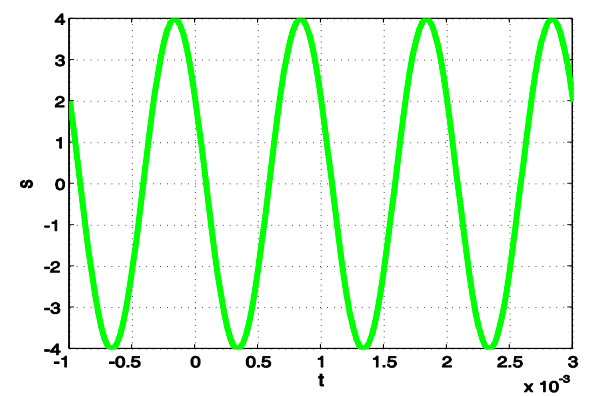
\includegraphics[width=0.5\textwidth]{harmonicky_signal_priebeh.png}
  \caption{Časový priebeh harmonického signálu $s(t) = 4\cos(2\pi \cdot 10^3 t + 0{,}3\pi)$}
\end{figure}

\textbf{Kvaziperiodický signál} je súčet harmonických signálov, pri ktorom aspoň dva kmitočty nemajú racionálny pomer -- inými slovami, nie je možné nájsť spoločný „základný" kmitočet, ktorého by boli všetky ostatné celistvými násobkami. Dôsledkom je, že signál sa nikdy presne nezopakuje, aj keď vizuálne vyzerá „takmer periodicky". Napriek tomu má, rovnako ako periodický signál, \textbf{čiarové (diskrétne) spektrum} -- energia je sústredená na konkrétnych diskrétnych kmitočtoch, nie rozložená spojito.

Príklad:
\begin{equation}
  s(t) = 2\cos(2\pi t) + 4\cos(t)
\end{equation}
kde pomer kmitočtov $2\pi / 1$ je iracionálne číslo.

\textbf{Neperiodický (aperiodický) signál} sa neopakuje vôbec -- buď existuje len v konečnom časovom úseku (impulz), alebo sa mení bez akejkoľvek pravidelnosti. Má \textbf{spojité spektrum} -- energia je rozložená plynulo po celej frekvenčnej osi.

\section{Výpočet výkonu}

Pre signál so zložitými hodnotami definujeme \textbf{normovaný okamžitý výkon} (pri $R=1\,\Omega$):
\begin{equation}
  p(t) = |s(t)|^2
\end{equation}

\textbf{Normovaná energia} signálu v intervale $\langle t_1, t_2 \rangle$:
\begin{equation}
  E = \int_{t_1}^{t_2} |s(t)|^2 \, dt
\end{equation}

\textbf{Stredný normovaný výkon} periodického signálu s periódou $T_1$:
\begin{equation}
  P_{\text{stř}} = \frac{1}{T_1} \int_0^{T_1} |s(t)|^2 \, dt
\end{equation}

Pre periodický signál vyjadrený Fourierovou radom $s(t) = \sum_{k=-\infty}^{\infty} c_k \exp(jk\omega_1 t)$ platí \textbf{Parsevalov teorém}:
\begin{equation}
  P_{\text{stř}} = \sum_{k=-\infty}^{\infty} |c_k|^2 = |c_0|^2 + 2\sum_{k=1}^{\infty} |c_k|^2
\end{equation}
Výkon teda možno vypočítať buď z časového priebehu (integrálom), alebo zo spektra (súčtom kvadrátov modulov koeficientov). Každý koeficient $|c_k|^2$ udáva, aká časť celkového výkonu pripadá na $k$-tú harmonickú zložku.

Pre aperiodický signál by bol stredný výkon nulový, pretože energia konečného impulzu sa pri delení nekonečne dlhým časovým intervalom blíži k nule. U aperiodických signálov preto hovoríme o \textbf{energii}, nie o výkone.

\section{Výpočet spektra}

\subsection{Fourierová rada -- periodické signály}

Každý periodický signál spĺňajúci Dirichletove podmienky možno rozložiť na súčet harmonických zložiek -- \textbf{Fourierova rada}:
\begin{equation}
  s(t) = \sum_{k=-\infty}^{+\infty} c_k \exp(jk\omega_1 t)
\end{equation}
Koeficienty $c_k$ (komplexné Fourierove koeficienty) sa vypočítajú:
\begin{equation}
  c_k = \frac{1}{T_1} \int_0^{T_1} s(t)\exp(-jk\omega_1 t)\,dt
\end{equation}
kde:
\begin{itemize}
  \item $k$ -- celé číslo, index harmonickej zložky,
  \item $\omega_1 = 2\pi/T_1$ -- základný uhlový kmitočet,
  \item $c_0$ -- jednosmerná (stredná) zložka signálu.
\end{itemize}
Množina koeficientov $\{c_k\}$ tvorí \textbf{frekvenčné spektrum} periodického signálu. Je to čiarové (diskrétne) spektrum -- kmitočtové zložky existujú len na celistvých násobkoch $\omega_1$.

\subsection{Fourierova transformácia -- aperiodické signály}

Pre aperiodické signály prechádzame k \textbf{Fourierovej transformácii} (FT):
\begin{equation}
  S(\omega) = \int_{-\infty}^{+\infty} s(t)\exp(-j\omega t)\,dt
\end{equation}
kde $S(\omega)$ je \textbf{spektrálna funkcia} (spojitá, komplexná). Inverzná FT:
\begin{equation}
  s(t) = \frac{1}{2\pi}\int_{-\infty}^{+\infty} S(\omega)\exp(j\omega t)\,d\omega
\end{equation}
Fyzikálna intuícia: keď zvyšujeme periódu periodického signálu $T_1 \to \infty$, čiary v spektre sa zhusťujú, až splynú do spojitého spektra.

\section{Typické príklady}

\subsection{Harmonický signál}

Harmonický signál $s(t) = C_1\cos(\omega_1 t + \varphi_1)$ má \textbf{čiarové spektrum} -- dve symetrické čiary na kmitočtoch $\pm\omega_1$ s amplitúdami $C_1/2$.

\begin{figure}[H]
  \centering
  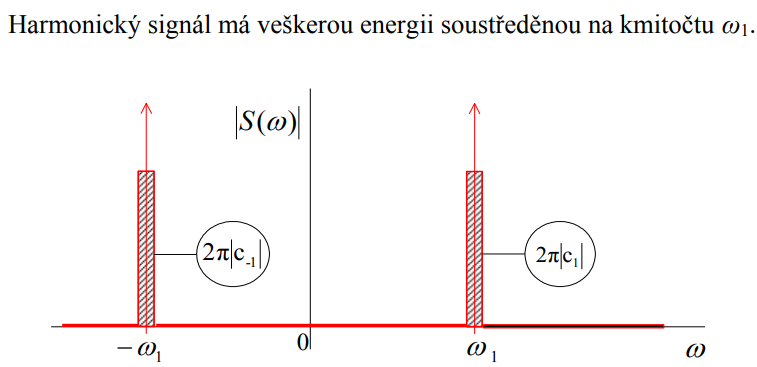
\includegraphics[width=0.82\textwidth]{harmonicky_signal_spektrum.png}
  \caption{Amplitúdové (čiarové) frekvenčné spektrum harmonického signálu -- dve symetrické čiary na $\pm\omega_1$}
\end{figure}

\subsection{Periodický sled obdĺžnikových impulzov}

Pre periodický sled obdĺžnikov (perióda $T_1$, šírka $\vartheta$, výška $D$) platí:
\begin{equation}
  c_k = D\frac{\vartheta}{T_1}\,\text{sinc}\!\left(\frac{\vartheta}{2}\,k\omega_1\right), \qquad
  \text{kde } \text{sinc}(x) = \frac{\sin x}{x}
\end{equation}
kde:
\begin{itemize}
  \item $c_k$ -- $k$-ty Fourierov koeficient,
  \item $D\vartheta/T_1$ -- jednosmerná hodnota (stredná hodnota signálu),
  \item $\vartheta/2 \cdot k\omega_1$ -- argument funkcie sinc, ktorý určuje kde sú nuly obálky.
\end{itemize}
Spektrum je čiarové, obálka čiar má tvar funkcie sinc. Prvá nula obálky je na $\omega_a = 2\pi/\vartheta$. Čím užší je impulz (menšie $\vartheta$), tým širšie je spektrum.

\begin{figure}[H]
  \centering
  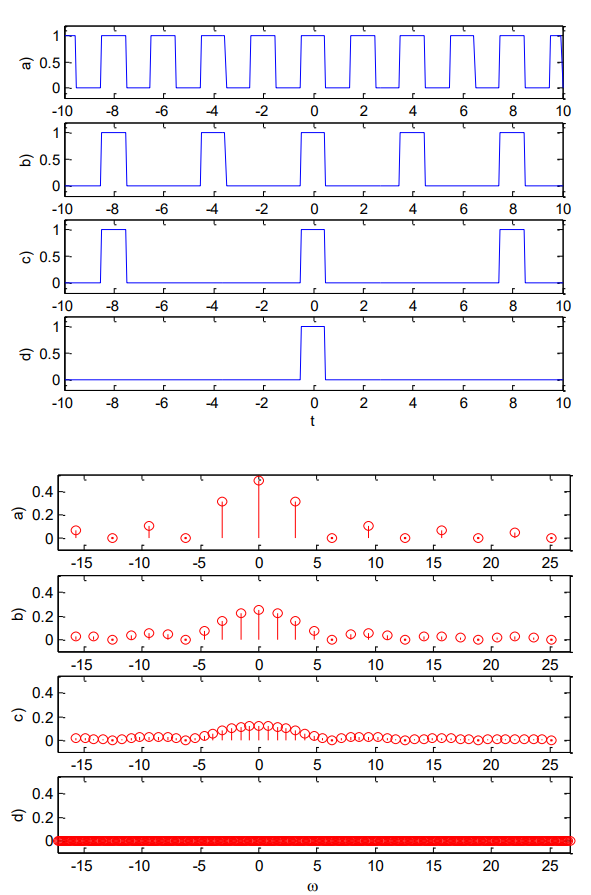
\includegraphics[width=0.82\textwidth]{periodicky_sled_obdlznikov_a_spektra.png}
  \caption{Periodický sled obdĺžnikových impulzov s parametrami $T_1$, $\vartheta$, $D$ a výpočet koeficientov Fourierovej rady}
\end{figure}

\subsection{Obdĺžnikový impulz}

Obdĺžnikový impulz so šírkou $\vartheta$ a výškou $D$, symetrický okolo $t=0$, má spektrum:
\begin{equation}
  S(\omega) = D\vartheta\,\text{sinc}\!\left(\frac{\vartheta}{2}\,\omega\right)
\end{equation}
kde:
\begin{itemize}
  \item $D\vartheta$ -- plocha impulzu (hodnota spektra pri $\omega=0$),
  \item $\vartheta/2\,\omega$ -- argument funkcie sinc.
\end{itemize}
Širší impulz $\Rightarrow$ užšie spektrum, užší impulz $\Rightarrow$ širšie spektrum. Asi 90\,\% energie leží v pásme $|\omega| < 2\pi/\vartheta$.

\begin{figure}[H]
  \centering
  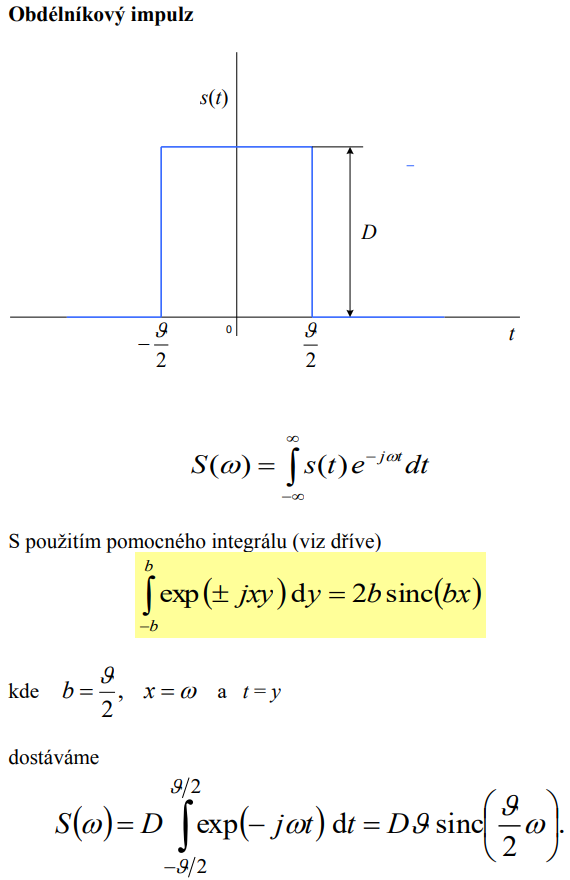
\includegraphics[width=0.7\textwidth]{obdlznikovy_impulz_spektrum_sinc.png}
  \caption{Obdĺžnikový impulz (vľavo) a jeho spojité amplitúdové spektrum tvaru sinc (vpravo)}
\end{figure}

\subsection{Harmonický impulz}

Harmonický impulz (rádiový impulz) je harmonický signál s krátkym trváním:
\begin{equation}
  s(t) = \begin{cases} A\cos(\omega_0 t) & \text{pre } |t| \leq \tau/2 \\ 0 & \text{inak} \end{cases}
\end{equation}
kde $A$ je amplitúda, $\omega_0$ je nosný kmitočet a $\tau$ je trvanie impulzu. Spektrum je sústredené okolo $\pm\omega_0$, s tvarom sinc. Čím dlhší impulz, tým užšie spektrum a tým viac sa blíži čiarovému spektru harmonického signálu.

\begin{figure}[H]
  \centering
  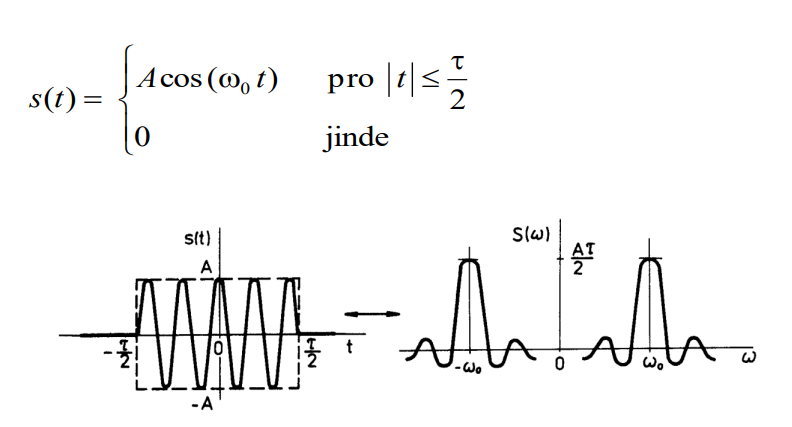
\includegraphics[width=0.82\textwidth]{harmonicky_impulz_spektrum.png}
  \caption{Harmonický (rádiový) impulz -- časový priebeh (vľavo) a jeho amplitúdové spektrum sústredené okolo $\pm\omega_0$ (vpravo)}
\end{figure}

% ============================================================
\chapter{Prevody medzi analógovými a digitálnymi signálmi; vzorkovanie, aliasing; rovnomerné a nerovnomerné kvantovanie; kvantovací šum}
% ============================================================

\section{Reťazec A/D prevodu}

Analogovo-číslicový (A/D) prevod prebieha v troch krokoch:
\begin{equation}
  s(t) \;\xrightarrow{\text{vzorkovanie}}\; \xrightarrow{\text{kvantovanie}}\; \xrightarrow{\text{kódovanie}}\; s(n)
\end{equation}

\section{Vzorkovanie}

\textbf{Ideálne vzorkovanie} spočíva v násobení spojitého signálu $s(t)$ radom Diracových impulzov so vzájomným odstupom $T$:
\begin{equation}
  s_v(t) = s(t) \cdot \sum_{n=-\infty}^{+\infty} \delta(t - nT)
         = \sum_{n=-\infty}^{+\infty} s(nT)\,\delta(t - nT)
\end{equation}

\begin{figure}[H]
  \centering
  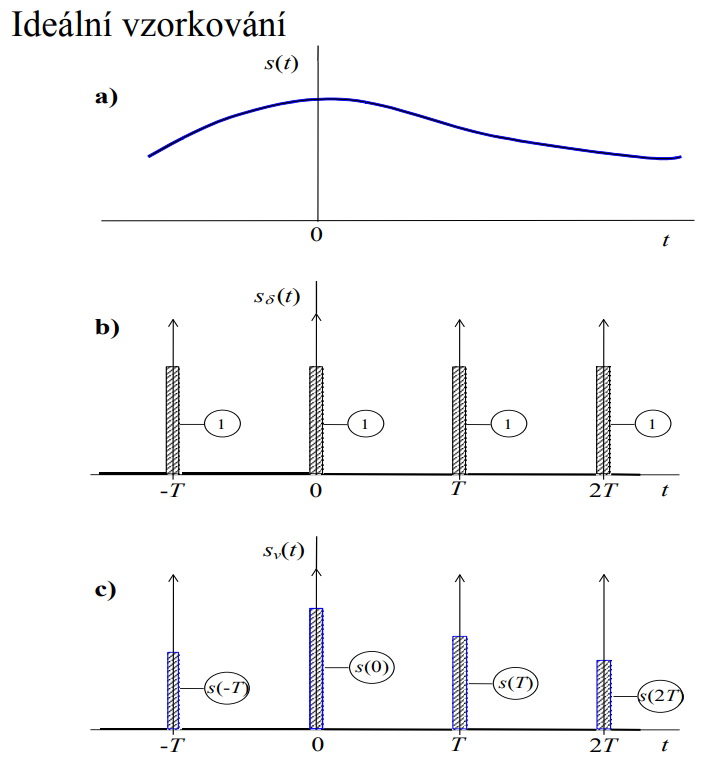
\includegraphics[width=0.7\textwidth]{idealne_vzorkovanie_casova_oblast.png}
  \caption{Ideálne vzorkovanie v časovej oblasti: a) pôvodný spojitý signál $s(t)$, b) sled jednotkových impulzov $s_\delta(t)$, c) vzorkovaný signál $s_v(t)$}
\end{figure}

Dôsledok v kmitočtovej oblasti: \textbf{periodizácia spektra} pôvodného signálu s periódou $\omega_1 = 2\pi/T$:
\begin{equation}
  S_v(\omega) = \frac{1}{T}\sum_{k=-\infty}^{+\infty} S(\omega - k\omega_1)
\end{equation}
Spektrum navzorkovaného signálu je teda nekonečná suma posunutých kópií pôvodného spektra, výškovo znížená faktorom $1/T$.

\section{Vzorkovací teorém}

\textbf{Vzorkovací teorém} (Nyquistov / Shannonov / Kotelníkův): Signál $s(t)$ so spektrom obmedzeným horným medzným kmitočtom $f_m$ možno jednoznačne vyjadriť postupnosťou vzoriek $\{s(nT)\}$, ak je splnená podmienka:
\begin{equation}
  \boxed{f_{\text{vz}} > 2f_m}
\end{equation}
kde $f_{\text{vz}} = 1/T$ je vzorkovací kmitočet a $f_m$ je horný medzný kmitočet spektra analógového signálu. Kmitočet $2f_m$ sa nazýva \textbf{Nyquistov kmitočet}.

\begin{figure}[H]
  \centering
  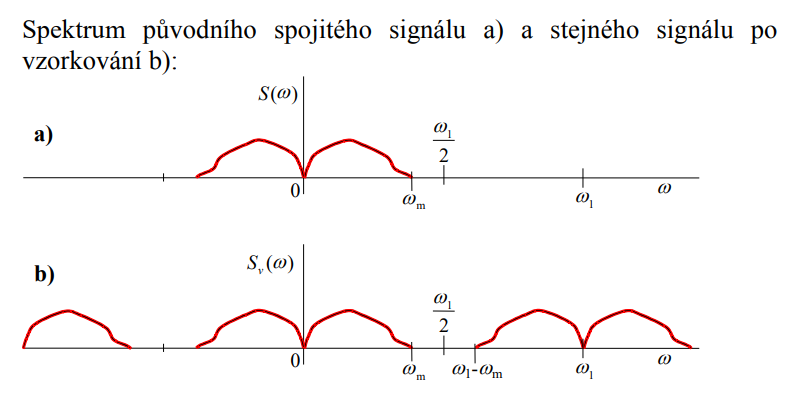
\includegraphics[width=0.82\textwidth]{spektrum_pred_a_po_vzorkovani_korektne.png}
  \caption{Spektrum pôvodného spojitého signálu $S(\omega)$ (hore) a spektrum navzorkovaného signálu $S_v(\omega)$ (dole) pri splnení vzorkovacieho teorému -- spektrá sa neprekrývajú}
\end{figure}

\section{Aliasing}

Ak podmienka vzorkovacieho teorému nie je splnená ($f_{\text{vz}} < 2f_m$), periodické kópie spektra sa začnú \textbf{prekrývať}. Tento jav sa nazýva \textbf{aliasing}. V kmitočtovej oblasti dochádza k sčítaniu zložiek z rôznych kópií spektra, čo spôsobuje nenahraditeľnú stratu informácie. V časovej oblasti sa aliasing prejaví zmenou tvaru rekonštruovaného signálu -- rôzne signály s rôznym kmitočtom produkujú rovnaké vzorky.

\begin{figure}[H]
  \centering
  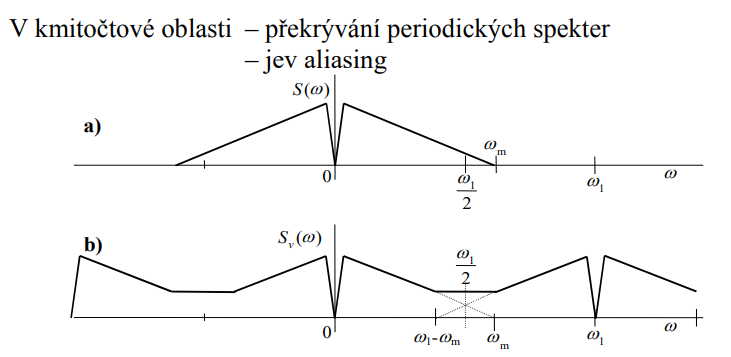
\includegraphics[width=0.82\textwidth]{aliasing_prekrytie_spektier.png}
  \caption{Aliasing -- prekrytie spektier pri nesplnení vzorkovacieho teorému: a) pôvodné spektrum $S(\omega)$, b) spektrum $S_v(\omega)$ s prekrytím (aliasing)}
\end{figure}

Obrana proti aliasingu: zvýšiť vzorkovací kmitočet $f_{\text{vz}}$, alebo pred vzorkovaním zaradiť \textbf{antialiasingový filter} (AAF, dolná priepusť s medzným kmitočtom $f_m < f_{\text{vz}}/2$), ktorý odreže frekvenčné zložky, ktoré by spôsobili aliasing.

\begin{figure}[H]
  \centering
  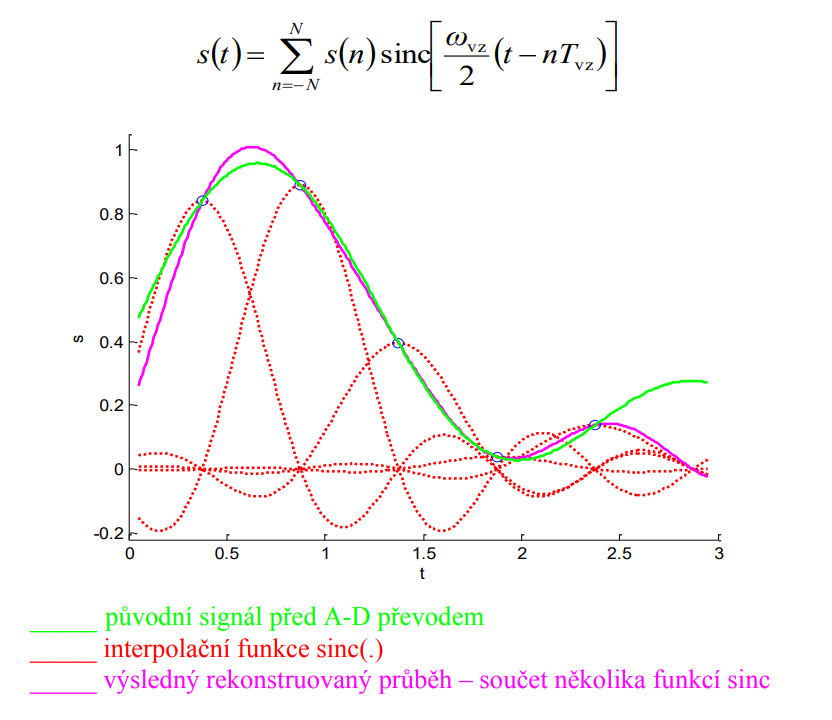
\includegraphics[width=0.82\textwidth]{rekonstrukcia_signal_zo_vzoriek.png}
  \caption{Vplyv antialiasingového filtra (AAF): a) spektrum signálu pred filtrovaním, b) spektrum navzorkovaného signálu po AAF -- spektrá sa neprekrývajú a rekonštrukcia je možná}
\end{figure}

\textbf{Rekonštrukcia signálu zo vzoriek:} Po správnom vzorkovaní možno pôvodný spojitý signál zrekonštruovať pomocou ideálnej dolnej priepuste s medzným kmitočtom $f_{\text{vz}}/2$. V praxi sa používajú rekonstrukčné (vyhladzovacia) filtre zaradené za D/A prevodník. Čím vyšší je vzorkovací kmitočet nad Nyquistovu hranicu, tým jednoduchší (menej strmý) rekonštrukčný filter postačuje.

\section{Kvantovanie}

\textbf{Kvantovanie} je zaokrúhlenie spojitých hodnôt vzoriek na konečný počet diskrétnych úrovní. Počet kvantovacích úrovní:
\begin{equation}
  N = 2^b
\end{equation}
kde $b$ je počet bitov na vzorku. Kvantovací krok (rozlíšenie):
\begin{equation}
  \Delta s = \frac{\text{Rozsah}}{2^b} = \frac{U_{\max} - U_{\min}}{2^b}
\end{equation}
kde:
\begin{itemize}
  \item $\Delta s$ -- veľkosť jedného kvantovacieho kroku,
  \item $U_{\max}, U_{\min}$ -- krajné hodnoty vstupného signálu,
  \item $b$ -- počet bitov (každý bit zdvojnásobí počet úrovní a zmenší $\Delta s$ na polovicu).
\end{itemize}

\begin{figure}[H]
  \centering
  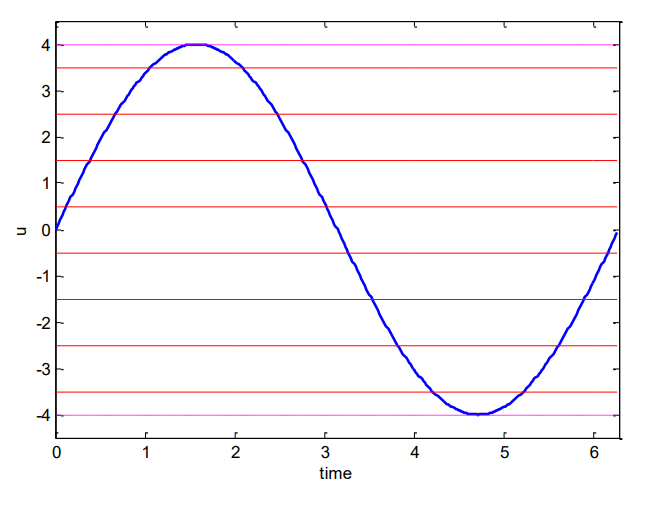
\includegraphics[width=0.7\textwidth]{kvantizacny_krok_pocet_bitov.png}
  \caption{Kvantovanie harmonického signálu -- sínusový priebeh s vyznačenými kvantovacími hladinami, $N = 2^b$ úrovní, kvantovací krok $\Delta s = \text{Rozsah}/2^b$}
\end{figure}

\section{Kvantovací šum}

Rozdiel medzi pôvodným signálom a kvantovaným signálom je \textbf{kvantovací šum}:
\begin{equation}
  r(t) = s(t) - s_{kv}(t)
\end{equation}
Šum $r(t)$ má pilovitý priebeh s amplitúdou $\pm\Delta s/2$.

\begin{figure}[H]
  \centering
  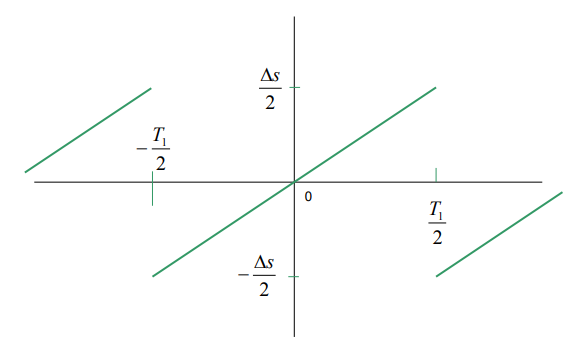
\includegraphics[width=0.82\textwidth]{kvantizacny_sum_priebeh.png}
  \caption{Kvantovací šum -- časový priebeh pôvodného signálu $s(t)$ a kvantovaného signálu $s_{kv}(t)$ (hore) a výsledný šum $r(t) = s(t) - s_{kv}(t)$ (dole)}
\end{figure}

Efektívna hodnota kvantovacieho šumu (odvodená pre pilovitý priebeh):
\begin{equation}
  R_{\text{ef}}^2 = \frac{1}{T_1}\int_{-T_1/2}^{T_1/2}\!\!\left(\frac{\Delta s}{T_1}t\right)^2\!dt
  = \frac{(\Delta s)^2}{12}
  \qquad\Rightarrow\qquad
  R_{\text{ef}} = \frac{\Delta s}{\sqrt{12}}
\end{equation}

\begin{figure}[H]
  \centering
  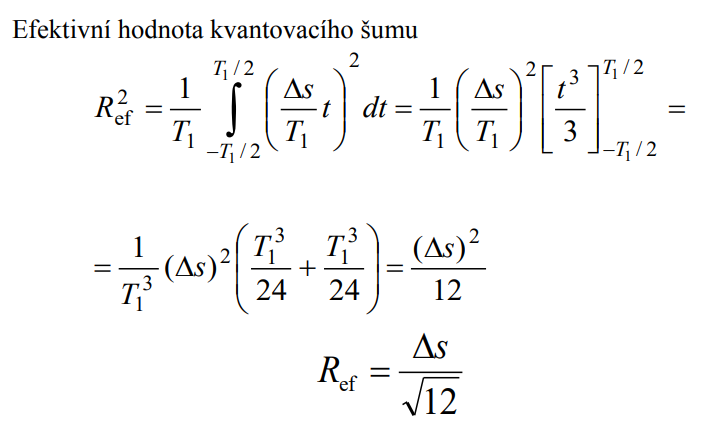
\includegraphics[width=0.7\textwidth]{kvantizacny_sum_odvodenie.png}
  \caption{Náhrada kvantovacieho šumu pilovitým priebehom -- základ pre výpočet efektívnej hodnoty $R_{\text{ef}} = \Delta s / \sqrt{12}$ a činiateľa zkreslenia}
\end{figure}

\textbf{Pomer signál/šum (SNR)} pre harmonický vstupný signál s amplitúdou $S_{\max}$ ($S_{\text{ef}} = S_{\max}/\sqrt{2}$):
\begin{align}
  \text{SNR} &= \frac{S_{\text{ef}}^2}{R_{\text{ef}}^2}
    = \frac{S_{\max}^2/2}{(\Delta s)^2/12}
    = \frac{6\,S_{\max}^2}{(\Delta s)^2}
\end{align}
Po dosadení $\Delta s = 2S_{\max}/2^b$ a vyjadrení v decibeloch dostaneme praktický vzorec:
\begin{equation}
  \boxed{\text{SNR} = 6{,}021\cdot b + 1{,}761 \quad [\text{dB}]}
\end{equation}
kde $b$ je počet bitov. Každý pridaný bit zvýši SNR o približne 6\,dB.

\section{Nerovnomerné kvantovanie}

Pri \textbf{rovnomernom kvantovaní} je $\Delta s$ konštantný pre všetky úrovne. Pre slabé signály je relatívna chyba kvantizácie väčšia ako pre silné signály -- to je nevýhoda napr. pri prenose reči, kde dominujú tiché pasáže.

\textbf{Nerovnomerné kvantovanie} rieši tento problém: jemnejšie kroky pre malé hodnoty, hrubšie kroky pre veľké hodnoty. Prakticky sa realizuje kombináciou \textbf{kompresora} a rovnomerného kvantizéra -- spolu tvoria \textbf{kompandér}.

\begin{figure}[H]
  \centering
  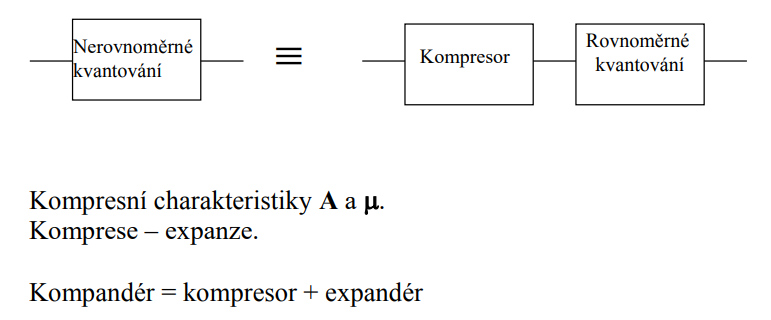
\includegraphics[width=0.82\textwidth]{nerovnomerne_kvantovanie_schema.png}
  \caption{Nerovnomerné kvantovanie -- schéma ekvivalencie: nerovnomerný kvantizér $\equiv$ kompresor + rovnomerný kvantizér}
\end{figure}

\section{Kódovanie}

\textbf{Kódovanie} je posledný krok A/D prevodu -- každej kvantovanej vzorke sa priradí binárne číslo (postupnosť núl a jedničiek). Najjednoduchší je \textbf{priamy dvojkový kód} (Natural Binary Code), kde každej úrovni zodpovedá jej binárna reprezentácia. Napríklad pre $b=3$ bity a $N=8$ úrovní: úroveň 0 = \texttt{000}, úroveň 5 = \texttt{101}, atď. Spôsob kódovania možno voliť podľa rôznych kritérií -- najčastejšie podľa dĺžky série alebo odolnosti proti rušeniu pri prenose (napr. Grayov kód, BCD).

\begin{figure}[H]
  \centering
  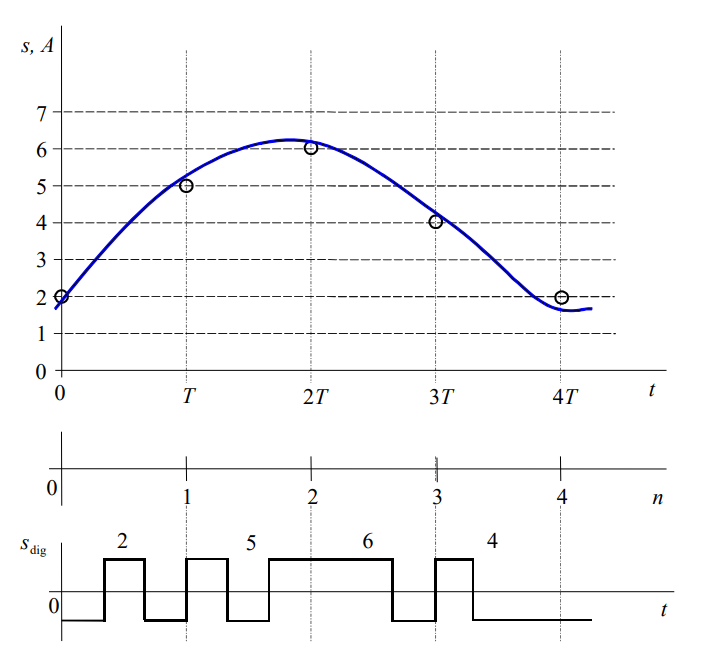
\includegraphics[width=0.82\textwidth]{AD_prevod_kodovanie.png}
  \caption{Kódovanie pri A/D prevode -- sínusový signál so vzorkami, číslicová postupnosť hodnôt vzoriek a priamy dvojkový kód pre $b = 3$ bity ($N = 8$ úrovní)}
\end{figure}

% ============================================================
\chapter{Lineárne a nelineárne systémy; vplyv nelinearity na spektrum; stabilné, kauzálne a časovo invariantné systémy; testovací signály}
% ============================================================

\section{Lineárne a nelineárne systémy}

Sústava je \textbf{lineárna}, ak platí \textbf{princíp superpozície} -- teda ak sústava reaguje na súčet viacerých vstupných signálov rovnako, ako keby sme sčítali jej odpovede na každý vstup zvlášť:
\begin{equation}
  ax_1(t) + bx_2(t) \;\rightarrow\; ay_1(t) + by_2(t)
\end{equation}
kde $a, b$ sú reálne konštanty, $x_1, x_2$ sú vstupné signály a $y_1, y_2$ sú zodpovedajúce výstupné signály. Princíp superpozície zahŕňa aj násobenie vstupného signálu konštantou (homogenita) aj sčítanie vstupov (aditivita).

\textbf{Nelineárna sústava} princíp superpozície nespĺňa.

\section{Vplyv linearity/nelinearity na spektrum}

\begin{itemize}
  \item \textbf{Lineárna sústava:} spektrum sa nezmení -- môžu byť potlačené alebo zosilnené niektoré existujúce zložky, ale \emph{nové kmitočtové zložky nevznikajú}.
  \item \textbf{Nelineárna sústava:} spektrum sa \emph{obohatí o nové zložky} -- harmonické skreslenie, intermodulácia. Na výstupe sa objavia zložky, ktoré na vstupe neboli.
\end{itemize}

\textbf{Príklad -- nelineárna sústava s kvadratickou charakteristikou:}

Na vstup sústavy $y(x) = a_1 x + a_2 x^2$ privedieme harmonický signál $x(t) = C\cos\omega_1 t$. Výstup:
\begin{align}
  y(t) &= a_1 C\cos\omega_1 t + a_2 C^2\cos^2\omega_1 t \notag \\
       &= \underbrace{\frac{1}{2}a_2 C^2}_{\text{jednosm.}}
         + \underbrace{a_1 C\cos\omega_1 t}_{\text{zložka }\omega_1}
         + \underbrace{\frac{1}{2}a_2 C^2\cos 2\omega_1 t}_{\text{nová zložka }2\omega_1}
\end{align}
Na vstupe bola jedna čiara ($\omega_1$), na výstupe sú tri: jednosmerná zložka, $\omega_1$ a nová $2\omega_1$.

\begin{figure}[H]
  \centering
  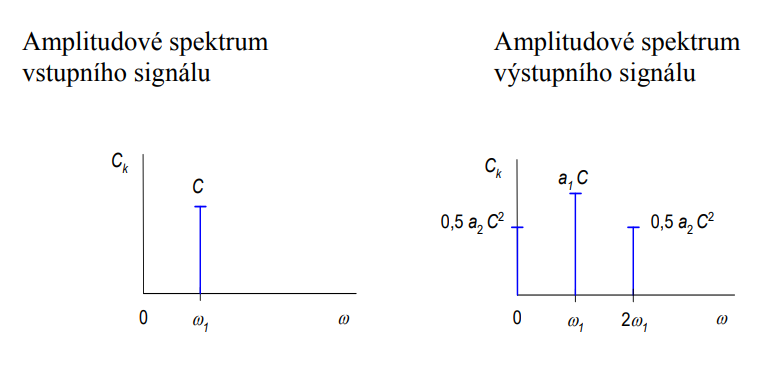
\includegraphics[width=0.82\textwidth]{nelinearny_system_amplitudove_spektrum.png}
  \caption{Amplitúdové spektrum na vstupe (jedna čiara na $\omega_1$) a na výstupe nelineárnej sústavy (jednosmerná zložka + $\omega_1$ + nová $2\omega_1$)}
\end{figure}

\section{Základné vlastnosti LSI sústav}

Sústava je \textbf{LSI} (lineárna, stabilná, časovo invariantná), ak spĺňa:

\begin{enumerate}
  \item \textbf{Linearita} -- platí princíp superpozície (viď vyššie).

  \item \textbf{Časová invariancia} -- posunutie vstupného signálu v čase o $\tau$ spôsobí rovnaké posunutie výstupného signálu:
  \begin{equation}
    x(t-\tau) \;\rightarrow\; y(t-\tau)
  \end{equation}
  Sústava sa teda nemení v čase -- jej parametre sú konštantné.

  \item \textbf{Stabilita} -- pre každý ohraničený vstup je výstup tiež ohraničený (podmienka BIBO -- Bounded Input, Bounded Output):
  \begin{equation}
    |x(t)|_{\max} \leq A < \infty \;\Rightarrow\; |y(t)|_{\max} \leq B < \infty
  \end{equation}

  \item \textbf{Kauzalita} -- výstup v čase $t_0$ nezávisí na budúcich hodnotách vstupu ($t > t_0$). Každá fyzikálne realizovateľná sústava je kauzálna.
\end{enumerate}

\section{Impulzná charakteristika a konvolúcia}

\textbf{Impulzná charakteristika} $h(t)$ je odozva LSI sústavy na \textbf{jednotkový impulz} $\delta(t)$ privedený na vstup:
\begin{equation}
  \delta(t) \;\rightarrow\; [\text{LSI}] \;\rightarrow\; h(t)
\end{equation}

Keďže každý signál možno rozložiť na sled impulzov rôznej váhy, stačí vedieť, ako sústava reaguje na jeden impulz -- teda poznať $h(t)$. Výstup pre ľubovoľný vstup $x(t)$ je potom \textbf{konvolúcia} vstupu s impulznou charakteristikou:
\begin{equation}
  y(t) = h(t) * x(t) = \int_0^{t} h(\tau)\,x(t-\tau)\,d\tau
\end{equation}

\section{Prechodová charakteristika}

\textbf{Prechodová charakteristika} $g(t)$ je odozva LSI sústavy na \textbf{jednotkový skok} $\sigma(t)$:
\begin{equation}
  \sigma(t) \;\rightarrow\; [\text{LSI}] \;\rightarrow\; g(t)
\end{equation}

Impulzná a prechodová charakteristika sú navzájom prepojené -- keďže jednotkový skok je integrálom jednotkového impulzu, platí:
\begin{equation}
  h(t) = g'(t) \qquad \Leftrightarrow \qquad g(t) = \int_0^t h(\tau)\,d\tau
\end{equation}

\section{Testovací signály}

Na testovanie a analýzu LSI sústav sa používajú štandardné \textbf{testovacie signály}:

\begin{itemize}
  \item \textbf{Jednotkový impulz} $\delta(t)$: Diracov impulz, konečná plocha v nulovom čase. Odozva naň je impulzná charakteristika $h(t)$ -- teda kompletný popis sústavy.

  \item \textbf{Jednotkový skok} $\sigma(t)$: signál skočí z 0 na 1 v čase $t=0$. Odozva naň je prechodová charakteristika $g(t)$. Definícia a varianty jednotkového skoku:

\begin{figure}[H]
  \centering
  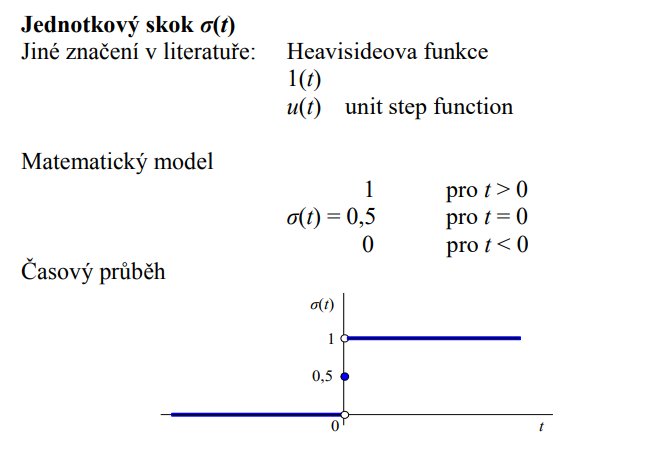
\includegraphics[width=0.82\textwidth]{jednotkovy_skok_priebeh.png}
  \caption{Jednotkový skok $\sigma(t)$ -- základný časový priebeh (hodnota 0 pre $t<0$, hodnota 1 pre $t>0$)}
\end{figure}

\begin{figure}[H]
  \centering
  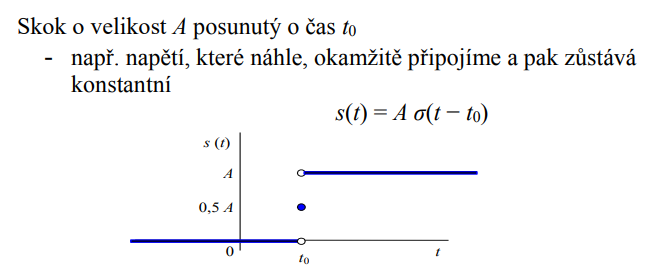
\includegraphics[width=0.82\textwidth]{posunuty_jednotkovy_skok_priebeh.png}
  \caption{Posunutý jednotkový skok $s(t) = A\,\sigma(t - t_0)$ -- skok o veľkosť $A$ posunutý o čas $t_0$}
\end{figure}

\begin{figure}[H]
  \centering
  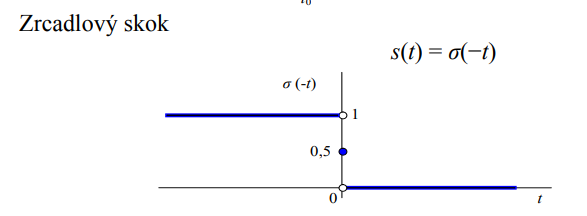
\includegraphics[width=0.82\textwidth]{zrkadlovy_skok_priebeh.png}
  \caption{Zrkadlový (časovo obrátený) skok $s(t) = \sigma(-t)$ -- zrkadlový obraz jednotkového skoku}
\end{figure}

  \item \textbf{Harmonický signál} $x(t) = C\cos(\omega_1 t + \varphi_1)$: najdôležitejší testovací signál v praxi. Odozva LSI sústavy na harmonický signál je \emph{opäť harmonický signál rovnakého kmitočtu}, ale so zmenenou amplitúdou a fázou. Závislosť amplitúdy a fázy od kmitočtu opisuje \textbf{frekvenčná charakteristika} $H(j\omega)$.

\begin{figure}[H]
  \centering
  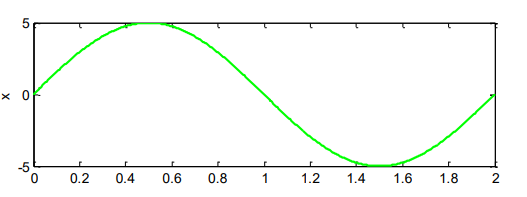
\includegraphics[width=0.82\textwidth]{harmonicky_testovaci_signal.png}
  \caption{Harmonický ustálený stav v LSI sústave -- vstupný harmonický signál $x(t)$ a výstupný signál $y(t)$ rovnakého kmitočtu so zmenenou amplitúdou a fázou}
\end{figure}

\end{itemize}

